\chapter{Testing}

Testing is an important aspect of any project. Even small projects can benefit from automated test to quickly check if a change has created an error somewhere in the code base. The larger a project is, the more fundamental testing becomes.

Three types of tests were outlined for this project in the requirements specification, unit tests, functional or end-to-end tests, and usability testing which included testing the application using different browsers. First testing within the server application will be considered, then tests necessary for the client side of the application will be explained.

\section{Server/API Tests}
The server provides the game logic, and resource API necessary for the game. Therefore, testing the server's functionality means making sure the API serves resources as expected and that the game logic responds as designed. Rails provides two types of tests that fit these needs: functional tests and unit tests respectively.

\subsection{Unit Tests}
The Rails framework provides model classes, each representing a type of record stored in the database. For example, the details of an application user will be stored as a record in the database, and so a User class  can be used to interact with the record and provide methods common to all users. Unit tests help to test each of these models in separation from the rest of the application in order to determine that its methods act as designed.

Unit testing began before the testing phase of the project was due to start. This was because as the application grew in complexity it became increasingly hard to check that areas of the application responded as intended. Unit tests helped to confirm that they did, or did not. So rather than being something tagged onto the end of the project, these tests actually served a useful role during development.

All models of the application have a respective unit test. Some of these are quite basic, because records that join two other tables may not require any logic of their own. In this case the tests establish that the joins between tables are set up correctly. Other test classes are extensive. In order to make the server application modular and to adhere to DRY (Don't Repeat Yourself) principals, as well as to make it more easily testable, much of the game logic was moved from the controller classes to the model classes. Some classes such as those representing games, cows, moves and cards had to test large blocks of logic requiring between ten and twenty tests each.
	
Two aspects of unit testing are worth a particular mention, as they involved learning new techniques. These are fixtures, and seeding random number generation.

Fixtures are a technology employed by Rails for quickly generating test data. A test database is used for test. This is emptied and loaded before each series of tests in order to ensure that tests are not disturbed by the results of other tests. Fixtures are a YML (Y.. Markup Language) representation of data that is loaded into the test database before running each test. So fixtures provide the 'truth' which tests are validated against.

This means that test data can be created quickly. However, certain relationships proved difficult to replicate using these fixtures. The positions that make up the board are stored in the database. In order to test the movement of rations, both the positions, and the joining records making the links between positions need to be supplied using fixtures. This type of one way relationship between records of the same table could not be done using fixtures, so while test positions were generated, none of them were connected to each other in the way necessary to build the board. Instead, positions had to be joined within the logic of the tests, before a test was carried out.

The second aspect that made testing more of a challenge was random number generation. The best example is dice rolls. When moving a food ration a user is presented with some randomly generated numbers between 1 and 6 to represent the roll of a dice. But how could this random generation be tested? Each time the dice rolls are generated they have a different result, by design, but tests need to know what their expected outcome is in order to test that the numbers have been generated as expected.

The solution was seeding the random number generator. Rails provides an easy method of doing this, and using a set-up utility before each test, the random number generator could be seeded so that it always gave the same result. Tests could then be built using these results.

So tests for all the application models were created, and application logic was updated until the tests representing the game requirements, passed. A full list of unit tests can be found in Appendix D.

\subsection{Functional Tests}
With the model logic working as expected, another important aspect of the server framework is the controllers, which serve the requests coming through the API. Controllers use the data models, but build on top of them, often adding an extra layer of functionality, or combination of model calls. This functionality needs testing. Because the API is stateless, and there is no particular order in which the API needs to respond, these serve as functional and integration tests.

An important aspect of these tests involved ensuring that unauthenticated users were denied the ability to access or amend resources that do not belong to them. This was not as straightforward as expected, because in order for game objects to be represented, a user may need read permission on another user's food ration, but should not be able to make changes to it. Different methods of authentication were therefore needed for GET requests than POST, PATCH and DELETE requests. This was achieved by testing that the user was authenticated or that the user was a player of a game for most GET requests. For most POST, PATCH and DELETE requests the controller checked that the user was the owner of the resource.

All the possible requests that can be made through the API were tested using functional tests. This helped to uncover some flaws in the API not considered in the design. One example is updating a player's moves. Ther controller checked for a parameter which indicates if the dice should be set. This was performed on the condition that a food ration had been chosen, but the controller did not check if the dice had been previously set. By creating tests, this small error was noticed and could be changed.

Functional testing also initiated the creation of standard responses for resources that were not found, or for unauthenticated requests. So the controller level of the application benefited from testing by becoming more uniform and having some lose ends removed. A full list of functional tests can be found in Appendix D.

\section{User Interface Tests}
Usability testing, from the beginning of the project, has been perceived as a vital part of the development of the application. This section explains how these tests progressed, and some of the benefits of performing them. Then automated client tests are considered.

\subsection{Usability Testing}
Usability testing began as soon as the project was in a state where a game could be played. Five groups of users helped to test the application in seven meetings held over a month. These comprised friends, family, computer science students, and the project client and supervisor. An attempt was made to get biologys students, one target audience, to test the game in a lecture setting, but no interest was shown. Despite this, the meetings held were extremely helpful, generating many suggestions.

To begin with players were registered by being entered into the database so that feedback could begin before registration was implemented. Some suggestions by users were put to effect straight away, if they were simple and fit with the current section of the project under development. Other suggestions were noted to be added later. Fixes that prevented the game being played were addressed as soon as possible.

Much of the feedback from users picked out logical flaws or bugs. These will not be focused on here, but are detailed, along with solutions, in Appendix D. It is more important to consider how user feedback impacted the overall design of the project and led to significant changes in the way the application data was presented.

Despite the time taken to create a good user interface design during the design phase of the project, the user interface needed many improvements. When users first tested the application, the main theme of their feedback was that controls were too complicated, and the game too difficult to pick up and play without knowing the rules before hand.

The aim of the project was to make a game that anyone can play. However, this goes beyond representing the existing board game as simply as possible. When playing a board game people expect to have to read a set of rules. Users of a web application, however, want to be able to pick up the rules as they go along. So not only do the controls need to be easy to find, but at the same time their location also needs to suggest how they are used, so that users do not have to read about how to make use of them.

User feedback, in Appendix D, suggested the best way to do this was to present only one task for the user to work on at a time. Instead of giving the user a page with many controls, let one action follow on from the other, with one decision to make at a time, while also making the impact of that decision obvious.

An example of the difficulties users had with understanding the controls is one person who missed the point of the game entirely when testing it. Because of a lack of information about how to play the game, this user clicked on buttons to finish various phases without once creating a food ration. So the game never presented the option of moving a food ration. As a short term solution a page of instructions was created explaining how to play the game.

A better solution was needed, however, for the game to fit its requirements of being easily playable in a classroom. A new user interface design was created based on user feedback and the one-task-at-a-time principal described above. This design had three main objectives that led to it's changes. 

The first concerned the fact that users found it difficult to associate the phase control buttons with the different screens that were displayed during a round. This is because unless the phases of the game are known, the names of the buttons referring to different phases were quite obscure. To avoid this confusion, cards and the cow digestive system can be shown on the same screen as shown in the diagram [reference]. This means that different phase screens are not needed. A user always has the same main view.

The second objective is to provide one task at a time. This is done by having just one command or question for the user to respond to at a time, and in a recognised place. While the first objective places all the information on one screen to view, this second objective prevents confusion from this information by focusing the user's attention to one place.

\begin{figure}[h]
\centering
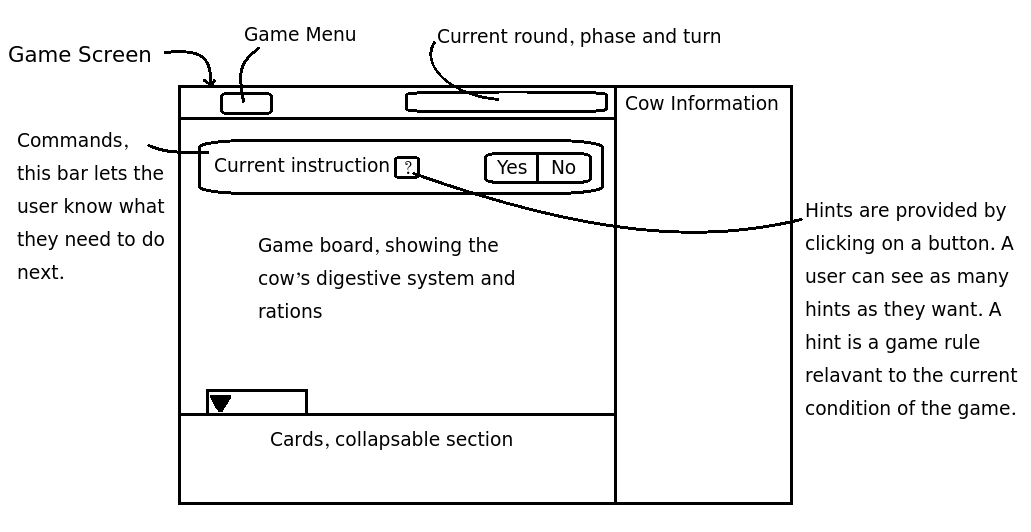
\includegraphics[width=3in]{Images/4/new-design}
\caption{A new proposed design, based on user feedback.}
\label{4_new_design}
\end{figure}

While the first two objectives focused on getting the user through the stages of the game, the third objective of the new design was to provide optional hints about some strategies a player could use as they make decisions during the game. This was planned in the form of a 'hints button'. Players could use this button as a way of asking for advice about what to do. The advice would depend, to some degree, on the current state of the game and the user's available cards.

\begin{figure}[h]
\centering
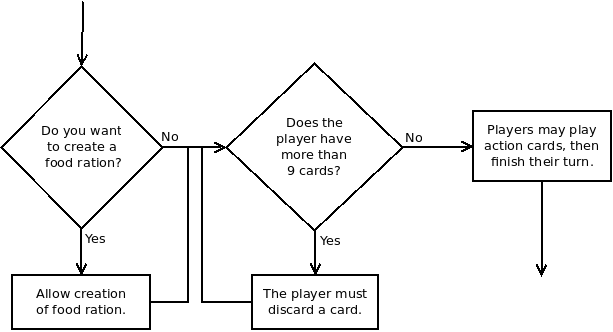
\includegraphics[width=6in]{Images/4/command-stages-cards}
\caption{The cards phase was broken up into these five stages. These stages are designed to improve usability, as a player will only have one task to perform at a time.}
\label{4_cards_commands}
\end{figure}

\begin{figure}[h]
\centering
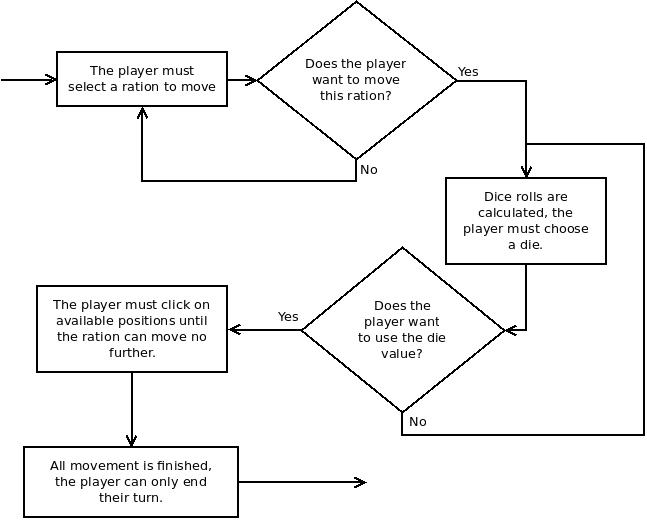
\includegraphics[width=3in]{Images/4/command-stages-movement}
\caption{The movement phase was broken up into these six stages. First they must choose and confirm a food ration, then they are presented with dice, and must move a food ration the number of positions shown on the dice they select.}
\label{4_cards_commands}
\end{figure}

Due to time constraints, only one objective of the new design were implemented: the second, single tasks at a time. This split the two main phases, the cards phase and the movement phase, into several sections, described in the diagrams below.

\subsection{Automated Testing}
On the client side automated testing is made possible through technologies such as Jasmine and Karma \cite{KarmaJasmine}. However, testing the client for the purposes of sifting the code base for bugs was not a priority of the project, as it had already been accomplished by the usability testing explained above. For maintenance, end-to-end testing would have been useful, but due to time constraints it was not included.

\subsubsection{Unit Testing}
AngularJS is modularised, making unit testing possible, and a good amount of documentation exists on how to begin. However, each module implemented for the project relied heavily on data returned from the API. Client side unit tests do not work well with asynchronous HTTP requests, because they require a stubbed service to be implemented that can respond instead of the server. As the modules of the project were thin layers dealing with the display of data returned from the server, any unit tests created would actually be testing the stubbed server API instead of the application, and so were not worth the time to create. 

\subsubsection{End-to-end Testing}
Instead of testing the data in separate modules, end-to-end testing attempts to mimic common uses of an application. If implemented these could be useful for maintenance of the code, as a way to ascertain if the functionality of the project remains the same after a significant code change. However, usability tests uncovered most issues that detailed tests would pick up, and so, with time constraints, these tests were left not implemented.